The \texttt{Model} package consists of all the classes managing data storage, filtering, and conversion.

\subsubsection{Model class} % Makes use of the rest of the classes in the Model package. The front-end class.
The \texttt{Model} class is the front-end class of the \texttt{Model} package (the only class which is directly connected to the \texttt{Controller} class). This is where the data structure is stored in a field and where the methods for filtering and converting data are called. The data structure is stored with the type \texttt{DataStructure}, which is an interface allowing us to easily switch between data structures.

\subsubsection{XMLReader class} % Reads in the data from an XML file of krax format and adds the content to a given data structure
This class reads data from an XML file of our KRAX format and converts it to instances of the \texttt{Edge} class (a simple class representing an edge on the roadmap), which are then added to a given data structure.

The \texttt{XMLReader} makes use of an external library, \href{www.xom.nu}{\texttt{xom}} (\url{www.xom.nu}), for reading the XML data.

\subsubsection{QuadTreeDS class} % The data structure of the application. Consists of several other classes to be explained here
The \texttt{QuadTreeDS} is the basis of the entire application. It is in an instance of this class that all data is stored after being read by the \texttt{XMLReader} class. In order for it to be used as our data structure, it implements the \texttt{DataStructure} interface.

The class consists of four instances of the \texttt{QuadTree} class (one for each type of road segment). A \texttt{QuadTree} consists of nodes, which has an x- and a y-coordinate (stored as \texttt{double}s) and a reference to an \texttt{Edge} object. Each \texttt{QuadTree} contains all edges of a designated type. Each \texttt{Edge} object is stored twice; both referenced to by the start- and end-coordinates of the edge.

Inserting a node into a \texttt{QuadTree} is a recursive process; the given node is compared to the root node, deciding which of the four children the given node is to be compared with next. This continues until a null-reference / a leaf is found.

Retrieving information is done using an instance of the \texttt{Interval2D} class (representing a rectangle), which again consists of two instances of the \texttt{Interval} class (each representing a line). This too is done recursively; it is checked whether the coordinates of the root node are within the given rectangle. If it is, it is added to a given collection of edges. It is then checked which of the subtrees might contain nodes within the rectangle, and for each that match, the same method is invoked, now with each of the matching children as the root. The call returns at null references.

Our implementation of the quadtree (including the \texttt{Interval} and \texttt{Interval2D} classes) is heavily based upon implementations from \url{algs4.cs.princeton.edu}.
\\
\begin{figure}[!h]
\centering
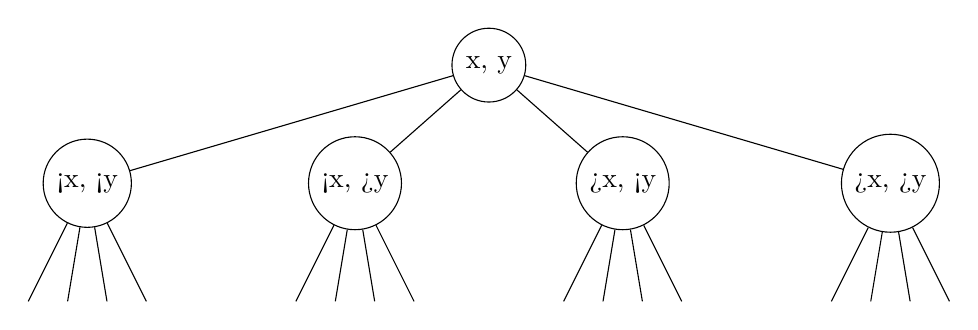
\begin{tikzpicture}
	[level 1/.style={sibling distance=34mm},
	level 2/.style={sibling distance = 5mm}]
	\tikzstyle{every node}=[circle,draw]
	\node {x, y}		
		child {
			node {<x, <y}
			child
			child
			child
			child
		}
		child {
			node {<x, >y}
			child
			child
			child
			child		
		}
		child {
			node {>x, <y}
			child
			child
			child
			child		
		}
		child {
			node {>x, >y}
			child
			child
			child
			child		
		}
	;
\end{tikzpicture}
	\caption{An illustration of the internal structure of the \texttt{Quadtree} data structure}
\end{figure}
\\
\subsubsection{FormatConverter class} % Converts from the data type pulled out of the data structure to the data type needed by the View package
The \texttt{FormatConverter} has static methods only, and only one public method. This methods takes an \texttt{ArrayList<Edge>} and converts it to the type \texttt{int[][][]} \\(\texttt{int[type][number of edges][edge coordinates]}).

The FormatConverter uses an instance of the Coordinates class to convert the given UTM32 coordinates to pixels as shown in the GUI.

\subsubsection{RoadDataCreator class} % Not directly part of the implementation, but the class used for converting the data from Krak to the krax XML format
The RoadDataCreator is not, strictly speaking, a part of the application (it is not used at runtime). It is a utility class, reading in the data supplied by Krak, writing it to an XML file of the KRAX format (once again using the external \href{www.xom.nu}{\texttt{xom}} library).

\subsubsection{The Graph}
Upon launching the application, the \texttt{Graph} class creates the two path finding graphs to be used by our path finding algorithm to find the fastest or the shortest path, respectively, between two given nodes.
	
The static \texttt{Graph} object itself contains \texttt{ArrayList} representations of each of these graphs. These will be referred to as graphs from now on. These graphs contain \texttt{Vertex} objects which have a position, some neighbouring vertices, and some adjacent edges (of the type \texttt{GEdge}). A \texttt{HashMap} for each of these two graphs is used to quickly access a vertex, given its id. Two \texttt{HashMaps} are used since each graph has its representation of each edge (the edges have different weights across the graphs). When searching for a path, the correct \texttt{ArrayList} and \texttt{HashMap} are returned, depending on whether the user requests the fastest path of the shortest path.

Furthermore, a third \texttt{HashMap} is used to keep track of each \texttt{Vertex's} adjacent \texttt{GEdges}.